\chapter{Results}
\label{chp:results} 

\section{Introduction}

This chapter presents how the robot and the supporting implementations were tested. Tests were performed on a simulated version of the robot and the real hardware. The software is inherently indifferent to weather the robot is simulated or real. However, it was still necessary to have some separate launch and configuration files for the simulated and hardware version. 

\section{Testplan}

The following tests will be carried out in the simulator, as well as in the real world. They will mainly focus on the navigation stack and \ac{RTAB-Map}. 

\begin{center}
	\begin{tabular}{ p{2.5cm} | p{7cm} }
		\multicolumn{2}{c}{Supporting Functionality}\\
		\hline
		\textbf{Evaluate} & Description\\
		\hline
	
	\end{tabular}
\end{center}

\begin{center}
	\begin{tabular}{ p{2.5cm} | p{7cm} }
	\multicolumn{2}{c}{Core Functionality}\\
\hline
	\textbf{Evaluate} & Description\\
	\hline
	\textbf{Multi Session Mapping} & Verify that the robot can rediscover areas which have been mapped in a previous mapping session.\\
	\textbf{Evaluate Loop Closure Detection} & As a core functionality in \ac{RTAB-Map}, it is critical to evaluate the loop closure mechanism.\\
	\textbf{Autonomous Navigation} & Perform a set of tests on the navigation stack. The tests should evaluate path planning with moving obstacles. Different parameters should be tested and evaluated. Observe how the robot handles narrow passages. Evaluate robustness of the navigation stack for this robot.\\
	\end{tabular}
\end{center}

\subsection{Supporting Functionality}

\section{Results}

\subsection{Simulations}

\begin{figure}[p]
	\centering
	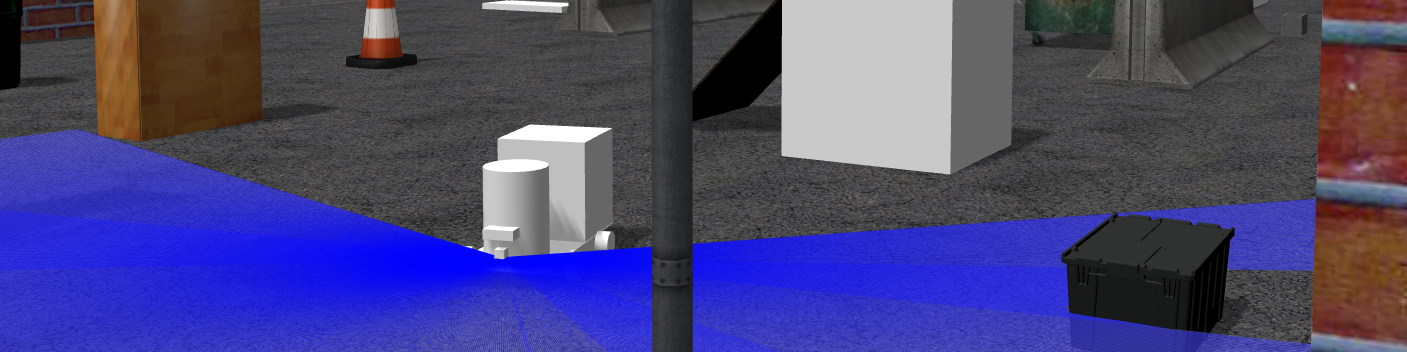
\includegraphics[width=1\textwidth]{gazebo2_cropped}
	\caption{The ''Asphalt'' world in Gazebo. }
	\label{fig:Incorrect_lc_detection}
\end{figure}

\begin{figure}[p]
	\centering
	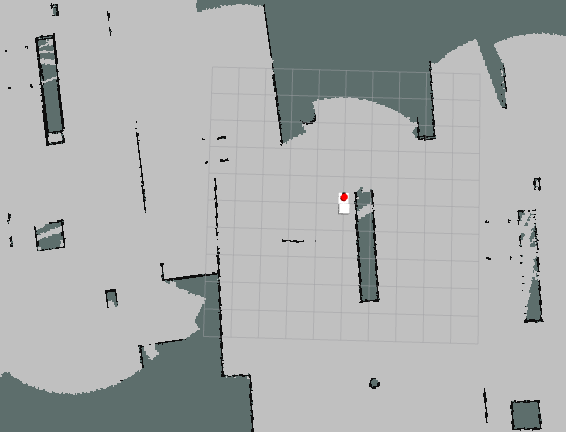
\includegraphics[width=1\textwidth]{Incorrect_lc_detection_cropped}
	\caption{An example of incorrect map merging. This case occurred in the ''Asphalt'' world simulated in Gazebo.}
	\label{fig:Incorrect_lc_detection}
\end{figure}

\begin{figure}[p]
	\centering
	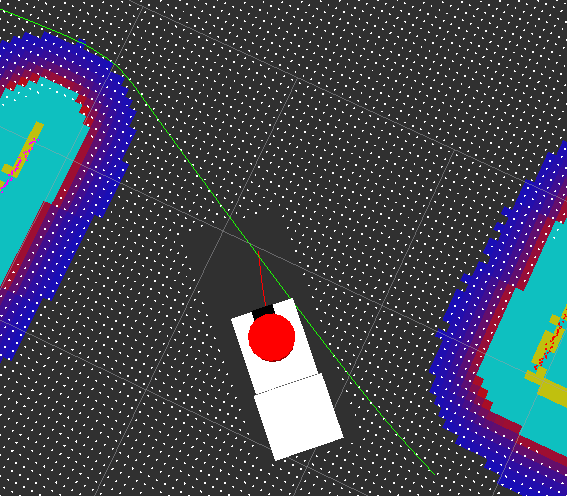
\includegraphics[width=1\textwidth]{planning_big_footprint_cropped}
	\caption{Nodes and topics for motion control. }
	\label{fig:big_footprint}
\end{figure}

\subsection{Live Testing}

Due to time constraints, it was no time to tune the parameters of \ac{RTAB-Map}.

\subsubsection{Safety Features}

\subsubsection{Loop Closure Detection}

\subsubsection{Multi Session Mapping}

\subsubsection{Navigating an Obstacle Course}

\begin{figure}
	\centering
	\begin{subfigure}[b]{0.46\textwidth}
		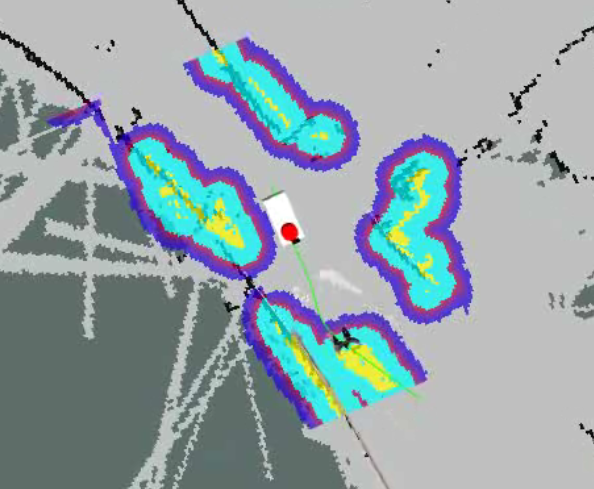
\includegraphics[width=\textwidth]{obstructed_plan}
		\caption{A person has moved into the path of the robot.}
		\label{fig:obstructed_plan}
	\end{subfigure}
	\begin{subfigure}[b]{0.472\textwidth}
		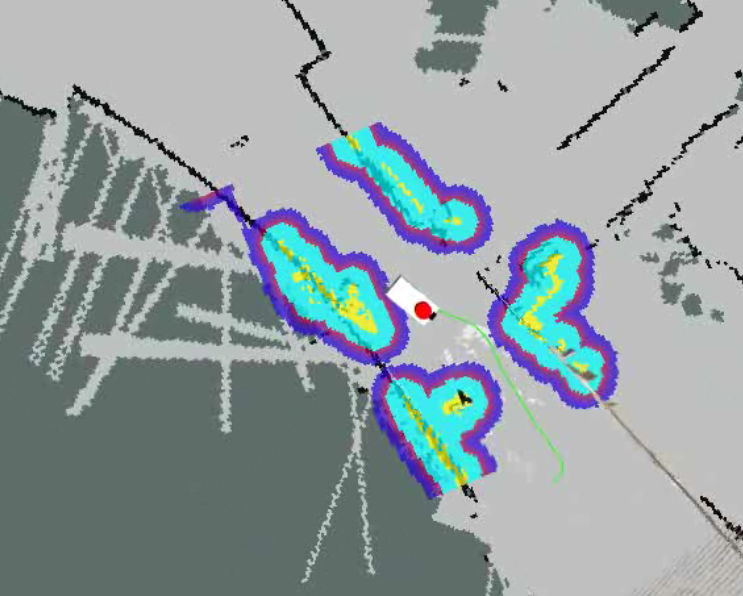
\includegraphics[width=\textwidth]{corrected_plan}
		\caption{A new path is planned, avoiding the new obstacle.}
		\label{fig:corrected_plan}
	\end{subfigure}
    \caption{Moving obstacle avoidance. The local cost map, shown as coloured spots on the occupancy grid, is based on real-time sensor data. }
\end{figure}

\subsubsection{Avoiding Moving Obstacles}






\section{Discussion}